\documentclass[12pt]{article}

\usepackage{sbc-template}

\usepackage{graphicx,url}

\usepackage[english]{babel}   
%\usepackage[latin1]{inputenc}  
\usepackage[utf8]{inputenc}  
% UTF-8 encoding is recommended by ShareLaTex
\usepackage{verbatim}
\usepackage{listings}
\usepackage{xcolor}
\usepackage{graphicx}
\usepackage{listings}
\usepackage[]{algorithm2e}
\usepackage{color}
\usepackage{amsmath}
\usepackage{amsfonts}
\usepackage{multirow}
\RestyleAlgo{ruled}
\usepackage{fancybox}
\usepackage{siunitx}

\graphicspath{ {Figures/} }

\newcommand\norm[1]{\left\lVert#1\right\rVert}
\definecolor{verde}{rgb}{0,0.5,0}
\DeclareMathAlphabet{\mathpzc}{OT1}{pzc}{m}{it}
%para customizar o código (ver https://en.wikibooks.org/wiki/LaTeX/Source_Code_Listings)
\lstset{language=C, %defina a linguagem usada no trabalho
              belowcaptionskip=1\baselineskip,
                breaklines=true,
                frame=false,
                xleftmargin=\parindent,
                showstringspaces=false,
                basicstyle=\footnotesize\ttfamily,
                keywordstyle=\bfseries\color{green!40!black},
                commentstyle=\itshape\color{purple!40!black},
                identifierstyle=\color{blue},
                stringstyle=\color{orange},
                numbers=left,
            }

\sloppy

\title{Virtual Reality 1}

\author{Dongho Kang, Jaeyoung Lim, Soomin Lee, Jaeryeong Choi}

\address{kangd@ethz.ch}

\begin{document} 

\maketitle

\section{Chapter 1: Introduction into Virtual Reality}

\subsection{Formation of Virtual Reality}

\subsubsection*{The concept of VR}

\begin{itemize}
	\item capture things and thoughts which elude human
	\begin{itemize}
		\item painting and stone sculpture (e.g. painting on the walls of cave) 
 		\item complex physical models (e.g. Newton's Law)
	\end{itemize} 
	\item \textbf{capture (copy) the reality \& portray the reality for the purpose of a better understanding}
\end{itemize}

\subsubsection*{VR before computer} 

\begin{itemize}
	\item The first projector : Laternae Magicae (17c) \textbf{Figure 1.2, page 1-2}
		\begin{itemize}
			\item optical system. a picture painted on a glass sheet and illuminated from behind with a candle
			\item monoscopic 
		\end{itemize}
	\item Mirror-based stereoscope (C. Wheatstone, 1832) \textbf{Figure 1.3, page 1-2}
		\begin{itemize}
			\item user can gain the impression of depth 
			\item very limited field of view
		\end{itemize}
	\item Panorama (R. Baker, 1787) \textbf{Figure 1.4, page 1-3}
		\begin{itemize}
			\item building (built at Leicester Square in London)  
			\item wider image than stereoscope: cylindrical images from height 10 ~ 14m, circumference 140m
			\item still image (no move)
		\end{itemize}
	\item Kaiserpanorama (19c) \textbf{Figure 1.5, page 1-3}
		\begin{itemize}
			\item moving panorama image
		\end{itemize}
	\item Head-Mounted-Display (Heilig \& Sutherland, 1960) \textbf{Figure 1.6, page 1-4}
		\begin{itemize}
			\item advances in the human-machine-interfacee, electronics and graphics hardware
			\item the rise of VR in the entertainment industries
		\end{itemize}
	\item Sensorama Simulator (M. Heilig, 1962) \textbf{Figure 1.7, page 1-4}
		\begin{itemize}
			\item one person arcade game (control of bikes and cars)
			\item stereovision / stereo sound / wind / realized scents 
			\item was not successful in the market
		\end{itemize}
	\item Waller Gunnery Trainer  \textbf{Figure 1.8, page 1-5}
		\begin{itemize}
			\item 5 cameras and 5 projectors
			\item used to train soldiers for the air force
		\end{itemize}
	\item Cinerama \textbf{Figure 1.9$\sim$11, page 1-6$\sim$7}
		\begin{itemize}
			\item 3 special cameras and 3 projectors (146\si{\degree} wide 55\si{\degree} hight) but some problems...
				\begin{itemize}
					\item stitch problem
					\item geometric distortion
					\item color temperature differences
					\item sync by hand (Theatre engineers)
					\item odd orientation of the actors (no eye contact)
				\end{itemize}
			\item cylindrical shape screen
		\end{itemize}
\end{itemize}

\subsection{The development of the computer}

\subsubsection*{Calculation and calculation machine}

\begin{itemize}
	\item The first scientific calculation: \textbf{abacus} 
	\item \textbf{Written calculation became popular (since 15c)}
		\begin{itemize}
			\item eased calculations and reduced the required time.
			\item lowered the failure rate.
		\end{itemize} 
	\item The first calculation machine (W. Schickardt, 17c) \textbf{Figure 1.16, page 1-12}
		\begin{itemize}
			\item add numbers up to 6 digits
			\item multiplication were possible. 
			\item toothed gears and slide rules. 
		\end{itemize}
	\item B. Pascal(1623 - 1662) \textbf{Figure 1.17, page 1-12}
		\begin{itemize}
			\item made money with calculation machine (the first one) 
			\item add and subtract numbers with 8 digits. 
			\item more than 50 pieces were produced. 
		\end{itemize}
	\item G. W. Leibniz (1646 - 1716) \textbf{Figure 1.18, page 1-12}
		\begin{itemize}
			\item introduced the machine suitable for all four basic calculation. 
		\end{itemize} 
	\item The calculating machines of 18c: more reliable, but became a piece of jewelry than a device for daily use \textbf{Figure 1.19, page 1-13}
	\item C. X. Thomas (1785 - 1870) \textbf{Figure 1.20, page 1-13}
		\begin{itemize}
			\item precise, efficient and ergonomic.
			\item "arithmometer": multiplied two numbers with 8 digits in 18 sec.
			\item more improved later 	
		\end{itemize}
	\item \textbf{Programmable calculation machines} (C. Babbage, 1792 - 1871)
		\begin{itemize}
			\item punched cards for programming. 
			\item could run the program autonomously.
			\item used steam machine and weights, but failed to realize his idea. 
		\end{itemize}
	\item \textbf{Calculation machine with electrical devices} (H. Hollerith, 1860 - 1929)
		\begin{itemize}
			\item \textbf{Figure 1.22, page 1-15}
			\item control mechanism activated by electrical devices (relays, motors ... ) with punched cards
			\item American Census in 1890: shorten the time for analysis 7 yrs $\rightarrow$ 1 yrs
			\item founded IBM
		\end{itemize}
\end{itemize}

\subsubsection*{Computer era}

\begin{itemize}
	\item Theoretical background of the first programmable electrical calculation machine (The first computer): \textbf{L. Couffignal and A. M. Turing}
	\item The first computer: \textbf{ZUSE Z3} by K. Zuse (1941)
		\begin{itemize}
			\item Z1 (didn't work) $\rightarrow$ Z2 (simple tests) $\rightarrow$ Z3 
			\item could handle 64 numbers with 22 digits. 
			\item 2600 relays and 8 line punched tape
			\item Z4 (1950s) worked at ETH 
		\end{itemize}	
	\item \textbf{The first encryptor \& decryptor}: Enigma vs Colossus (1941)
		\begin{itemize}
			\item MARK 1 (1943) in US
			\item MARK 2 (1944) in US
		\end{itemize} 
	\item \textbf{The first electronical computer, ENIAC (1946)} \textbf{Figure 1.25, page 1-16}
		\begin{itemize}
			\item J. P. Eckert, J. Mauchley and H. H. Goldstine
			\item 18000 tubes, 1500 relays, 1000 capacitors and 6000 switch.
			\item very fast... 0.0002 sec for addition, 0.0028 sec for multiplication 
		\end{itemize}
	\item \textbf{Transistor} invented (1948) \textbf{Figure 1.26, page 1-17}
		\begin{itemize}
			\item smaller, faster, less heat, longer life cycle ...
			\item manufactured automatically 
			\item \textbf{switch: relays $\rightarrow$ tubes $\rightarrow$ transistor}
		\end{itemize}   
	\item \textbf{single chip computer(CPU)} (Integrated Circuits) 
		\begin{itemize}
			\item 4-bit processor INTEL and Texas Instrument in 1970
			\item 8-bit (1972), 16-bit (1978) ... now 32 bit / 64 bit
		\end{itemize}
	\item \textbf{Personal Computer (PC)}
		\begin{itemize}
			\item because of IC, the size of computers could be drastically reduced
			\item Kenbak1 (1971): the first single chip computer
			\item ALTAIR 880 (1974): mass market
				\begin{itemize}
					\item \textbf{Basic}: a new programming language developed for ALTAIR
				\end{itemize}
			\item Apple II \& Commodore PET: the first commercial success
			\item IBM PC became very popular
		\end{itemize}
	\item SGI were used for high-performance computer graphics: Virtual Reality...
\end{itemize}

\subsubsection*{Moore's law and the development of computer}

\begin{itemize}
	\item \textbf{Moore's law} (1965): \textbf{the amount of transistors} in a computer is doubled all 18 months. \textbf{Figure 1.34, page 1-22}
	\item but also the required space for the transistors becomes smaller and smaller. i.e. \textbf{the available memory per chip} is increases: x4 every 3 yrs
	\item \textbf{chip size} also increases: x2 every 10 yrs 
	\item \textbf{CPU speed} increases: x2 every year
\end{itemize}

\subsection{Definitions}

\begin{itemize}
	\item Reality (exist): real object $\gg$ virtual object
	\item Mixed Reality 
		\begin{itemize}
			\item Extended Reality (Augmented Reality): real obj $>$ virtual obj
			\item Extended Virtuality (Augmented Virtuality): real obj $<$ virtual obj
		\end{itemize}
	\item Virtual Reality (non exist): real obj $\ll$ virtual obj
	\item \textbf{Note: Figure 1.39, page 1-25}
\end{itemize}

\subsubsection{Extended Reality (augmented reality)}

\begin{itemize}
	\item \textbf{real object $>$ virtual object}
	\item the computer generated objects are characterized by the fact but usually differ from reality in scale, shape or color.
	\item e.g. AR on copy machine: indicate parts to be fixed  
\end{itemize}

\subsubsection{Extended Virtuality (autmented virtuality)}

\begin{itemize}
	\item \textbf{real object $<$ virtual object}
	\item comparing to AR, virtual objects are much more detailed and fit much better to reality.
	\item e.g. Reconstruction of ruins \textbf{Figure 1.40}
\end{itemize}

\subsubsection{Virtual Reality}

\subsubsection*{Definition}

\begin{itemize}
	\item Former Definition: a possible or considered reality, \underline{which is not available yet.}
	\item Complete Definition: \textbf{"Virtual Reality is a computer generated, interactive and three-dimensional environment, in which the user is completely immersed"}
		\begin{enumerate}
			\item a fictive and non-real world (e.g. TV, movie, dream are fictive and non-real world)
			\item "cybernetic room" or "cyberspace": controllable and manageable room, in which information is processed. (e.g. chess, board games)
			\item generated by computer, using specialized program: imaginary reality can only be reached by processing numerous infos. 
		\end{enumerate}
\end{itemize}

\subsubsection*{The VR reference model}

\begin{itemize}
	\item \textbf{Figure 1.41, page 1-27}
	\item Three component (three axis)
		\begin{itemize} 
			\item interaction (none $\rightarrow$ interactive $\rightarrow$ immersive)
			\item semantics of data (none $\rightarrow$ static $\rightarrow$ dynamic)
			\item presentation (single event $\rightarrow$ sequence of events $\rightarrow$ real time)
		\end{itemize}
	\item optimal VR application $=$ \underline{immersive interaction} $+$ \underline{dynamic semantics} $+$ \underline{real time presentation} 
	\item Note, but not each VR application requires the maximum amount of all three criteria.
\end{itemize}

\section{Chapter 2}

\newpage
\section{Chapter 3: Introduction into Computer Graphics}

\subsection{Introduction}

\begin{itemize}
	\item Quick development in computer graphics: from an expensive toy to an attractive research field
		\begin{itemize}
			\item main reason: human receives most of the information through the visual perception channel
			\end{itemize}
	\item Rapid development concerning hardware, software, and applications
		\begin{itemize}
			\item graphics can be easily accessed and understood by different cultures/people/languages (high synergy among people)
		\end{itemize}
\end{itemize}

\subsection{Why do we need Computer Graphics?}

\begin{itemize}
	\item The representation of texts is also a special form of graphics
	\item Human being seems to have a better access to images and pictures than letters and numbers
		\begin{itemize}
			\item e.g. complex simulation results by visualization, logo of a company
		\end{itemize}
\end{itemize}

\subsubsection*{Computer Graphics and Picture Recognition}

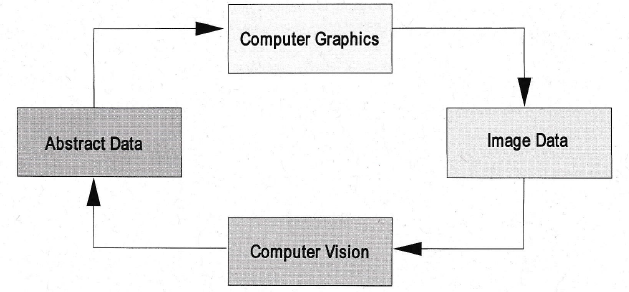
\includegraphics[scale=0.6]{3_1}

\begin{itemize}
	\item When a human perceives the surrounding world, the brain generates an abstract "data model"
	\item Computer Vision: extract relevant data out of existing graphics or images
	\item Computer Graphics: display the data
\end{itemize}

\subsection{Applications of Computer Graphics}

\subsubsection*{CAD}

\begin{itemize}
	\item Construction (Functional Design)
	\begin{itemize}
		\item the requirements to an assembly part are well defined by function and dimension
		\item all drawings on a CAD system are a complex relationship between dimensions, constraints, and material properties, which describe a part very well
	\end{itemize}
	\item Design (Aesthetic Design)
	\begin{itemize}
		\item do not focus on the dimension of a part, but factors like ergonomics or aesthetics
		\item many suppliers of design software try to combine the relatively free aesthetic design field with the very compulsory functional design, but hasn't been successful due to difficult exchange of data between both worlds
	\end{itemize}
\end{itemize}

\subsubsection*{Gaming}
\begin{itemize}
	\item Caused a significance increase of graphic performance in the private computer sector
	\item Cheap components and fast, high- quality software were developed due to the growing demands of players and the competition of the industry
\end{itemize}

\subsubsection*{Visualization}

\begin{itemize}
	\item Visualization is the ancestor of 3D computer graphics
	\item \textbf {Definition: Visualization addresses special properties of human perception to visualize and to represent information, which is extracted from large amount of data}
	\item Visualization intends to:
	\begin{itemize}
		\item display structures, models, trends, anomalies, and relationships
		\item give an overview of large amounts of data
		\item give support by means of an easy modification of parameters when searching for interesting regions in a large data field
	\end{itemize}
	These points can be summarized in the mantra of Ben-Shneiderman:
	\begin{center}
	\textbf{overview, zoom-in, filtering, details on request}
	\end{center}
	Thus, a good visualization has the following properties:
	\begin{itemize}
		\item it prevents misinterpretation and ambiguity
		\item it optimizes the perception of subtle properties
		\item it allows displaying more data at a time
	\end{itemize}
	\item Typical data sets which need to be visualized very often:
	\begin{itemize}
		\item MRI (the density can be visualized by different colors and transparencies)
		\item CFD (the location and the direction of movement of points with 6 DOF, color and particles, size or shape can display the information)
		\item Financial Data (display in a diagram, so that a user can see correlations between variables)
		\item CAD (3D data with additional information for edges, corners, surfaces, and surface properties. Complex data structures are used because the data is used not only for visualization but also for other processes. Complexity of the models strongly depends on the display quality)
		\item Statistical data sets (the correlation between different parameters only can be seen through visualization)
	\end{itemize}
	\item Different kinds of visualization in the following table. The different categories do overlap in many cases, "Illustration" has an exceptional position since it can be used everywhere
\end{itemize}

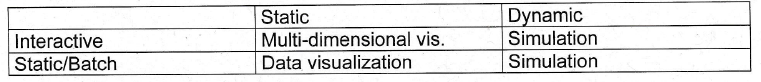
\includegraphics[scale=0.7]{3_8}

\begin{itemize}
	\item Data Visualization
		\begin{itemize}
			\item The most common way would be Excel-like presentation (e.g. pancake diagram, 3D graphs)
		\end{itemize}
	\item Cybernetic Visualization (Simulation)
		\begin{itemize}
			\item The main interest in the visualization of a cybernetic application: speed and possible detection of errors and irregular behavior of the simulated system
			\item The classical way: showing data in a 2D graph as a time-dependent value
		\end{itemize}
	\item Multi-dimensional Visualization
		\begin{itemize}
			\item when much data has to be displayed simultaneously within one image
			\item every point in the space can represent 3 independent values + color, line thickness, transparency, different shapes, etc.
			\item other ways exist but a compromise has to be made concerning the simplicity (e.g. switch between different data visualization planes on any given point of a curve or shape)
		\end{itemize}
	\item Statistics
		\begin{itemize}
			\item typically statistics contain many different values for one single measurement.
			\item the visualization's task is showing possible correlations among the different values
			\item only valid for the given constraints
		\end{itemize}
\end{itemize}

\subsubsection*{Illustration}

\begin{itemize}
	\item Illustrations are 2D add-ons to a 3D object. They contain much additional information about the 3D representation.
	\item GUIs
		\begin{itemize}
			\item the most important means of communication between the user and the computer
			\item the most important input device is the mouse
			\item basic idea of GUI: pointing on an object is one of the easiest gestures of a human being
			\item within the GUI an icon is a small image, which is a representation for a program sequence or for the content of a defined type (they made working with a computer much faster and more comfortable because people can just 'click' on them instead of entering complex instructions)
		\end{itemize}
	\item Fonts
		\begin{itemize}
			\item within the visualization, text is used to assign abstract contents like titles, classifications, or dimensions to a graphical object
			\item Typesets and fonts are the medium of text (based on typography and applications)
		\end{itemize}
	\item Layout
		\begin{itemize}
			\item By placing graphical elements on a surface, the underlying information is structured more clearly and more detailed
			\item typical applications: windows-based desktops such as MacOS, Windows (e.g. word wrap)
			\item Another kind of layout is characterized by the given application (e.g. simulation of operation elements in a car- the ergonomic placement of the elements is essential for the overall handling of the vehicle)
		\end{itemize}
	\item Drawings
		\begin{itemize}
			\item very often used to visualize abstract situations
			\item e.g. organization charts or flowcharts, manuals
		\end{itemize}
	\item Instructions
		\begin{itemize}
			\item instructions consist of a mixture of text, graphical visualization, photos, etc.
			\item very often they visualize products in an abstract and simplified way
			\item e.g. service manuals, assembly manuals
		\end{itemize}
\end{itemize}

\subsection{Definition of 3D Graphics}

\begin{itemize}
	\item Definition of 3D graphics: \textbf{The field 3D graphics deals with the generation of 3D objects and their representation on a two-dimensional surface(e.g. a screen)}
	\item the main focus is on projection and visualization of a 3D space on a 2D surface of any kind
	\item example of 3D graphic devices: video camera, photo camera
	\item main characteristics of 3D graphics:
	\begin{itemize}
		\item data acquisition / data transfer / storage
		\item transformation / processing
		\item data display on 2D
		\item input and output
	\end{itemize}
	\item simple pipeline for data processing: \\
		$\rightarrow$ Definition of geometry as digital data \\
		$\rightarrow$ Processing and transformation of data \\
		$\rightarrow$ Transformation of data to 2D \\
		$\rightarrow$ Display of the results on a screen
\end{itemize}

\subsection{Rendering Pipeline}

\begin{itemize}
	\item The rendering pipeline is the basis for almost every application in computer graphics
	(can be slightly modified for special applications such as augmented reality)
	\item The simplest form of the rendering pipeline: \\
	$\rightarrow$ Processing and transformation of data \\
	$\rightarrow$ Transformation of data to 2D \\
	$\rightarrow$ Display of the results on a screen
	\item transformation / processing: modify the original data in such a way that it can be displayed well on a 2D surface. contains data modified by the user e.g. modified viewing angle onto the geometry
	\item transformation of data to 2D: all modified data has to be transformed onto the 2D surface. e.g. removal of hidden objects or surfaces, transferring a curved surface into triangles, or the integration of illumination models
	\item input/output: reduce the amount of data so that the image can be optimally displayed on the output device (due to limitation in resolution)
\end{itemize}

\subsection{Definition of Geometry in the Computer}

\begin{itemize}
	\item Algorithms for a geometric representation of curves and bodies were developed in order to model hulls, car bodies, and fuselages
	\item B\'ezier developed a CAD-system (further developed into the 'UNISURF' system later on), close approximation to geometry
	\item In order to define geometry, the information should be sufficient but not redundant
	\item It can be distinguished between volumetric and surface models
\end{itemize}

\subsubsection*{Discrete Definition of Surfaces}
\begin{itemize}
	\item Cloud of Points:
	\begin{itemize}
		\item the simplest model, every point of the cloud is defined by its coordinates
		\item The point cannot be rendered(no information on color or texture) and there is no connectivity among the points(separate parts cannot be selected in the model)
		\item 3D-scanner typically provides a cloud of points
		\item difficult to create a good surface out of the clouds of points because the acquired data is noisy and erroneous
	\end{itemize}
	\item Polygons, Tessellation:
	\begin{itemize}
		\item Tessellation is a method for defining or generating a mesh of geometric basic elements(polygons), which approximate a complex surface
		\item Polygon, especially triangle, is one of the most important basic elements of computer graphics
		\item "triangulation": the process in which a free-form surface is transformed into triangles (The mesh approximates the surface by triangles and reduces the complexity)
		\item additional data has to be considered when rendering (e.g. perpendicular of a surface)
	\end{itemize}
	\item Polystrips
	\begin{itemize}
		\item when a point is added to a triangle, a second triangle will be generated
		\item advantage: a large amount of surfaces can be generated by a very low amount of data
		\item stored in two tables: the point(vertex) table with all coordinates of the triangle's corners and the strip table with all coherent triangles
		\item details could be lost since any curve is approximated by straight lines of different lengths
		\item many times the triangulation is done at a very late stage in rendering because often working with mathematically exact representations of the geometry is required
	\end{itemize}
\end{itemize}

\subsubsection*{Mathematical Description of Geometries}

\begin{itemize}
	\item Typically, the surfaces of objects are represented by approximating functions
	\item A parametric representation is used for the approximation or interpolation of these surfaces (e.g. parametric polynomials - B\'ezier, B-Spline)
	\item Surface models are mainly used- drawback: there are no relationships among the individual parts of the surface (The individual surfaces are not correlated with an object and thus the shape of an object is a question of interpretation)
	\item possibilities for the mathematical description of curves and surfaces: explicit, implicit, parametric
	\begin{itemize}
		\item explicit: only one value for y is associated with the variable x\\
		thus problems arise for closed curves or objects\\
		it is not invariant to rotations\\
		only a few geometries can be described by such an explicit notation, rarely used
		\item implicit: typically implicit equations have more solutions than required and thus additional constraints have to be considered\\
		also rarely used in virtual reality
		\item parametric: the most common descriptive form\\
		no equivocations could occur, the definition is invariant to rotations\\
		infinite slopes can be described by tangential vectors which are finite\\
		typically consist of rational polynomials of the nth degree, most frequently cubic polynomials are used\\
		any point of the geometry can be exactly determined by mathematical functions (particular interest for CAD)
	\end{itemize}
	\item B\'ezier splines:
	\begin{itemize}
		\item first used in shipyards
		\item goal: interconnect given points by a smooth line
		\item points that approximate the curve are called "control points"
		\item mathematical function that delivers the result is named "base function", guarantees that the requirement for continuity in the control points is kept by interpolation or approximation
	\end{itemize}
	\item approximation: a curve approximates given control points / interpolation: the calculated curve has to meet the control points exactly; important in both cases that continuity is fulfilled
	\item "parametric continuity":
	\begin{itemize}
		\item represented by the letter C and its exponent i which defines the degree of the i\textsuperscript{th} derivation \\
		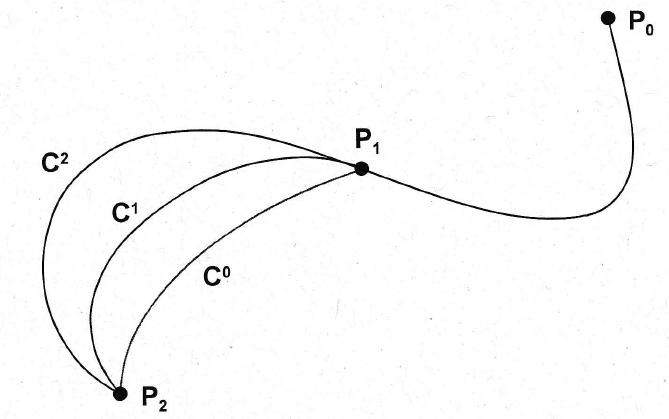
\includegraphics[scale=0.5]{3_24}
		\item C\textsuperscript{0} continuity: guarantees that the curve is not interrupted, but it could happen that a curve is not smooth in the point P1 but has an edge instead
		\item C\textsuperscript{1} continuity: the first derivation is continuous, all tangent vectors in the point P1 have the same slope, the curve is smooth at the point P1 (continuity of tangents)
		\item C\textsuperscript{2} continuity: the second derivation is continuous, the curve looks even smoother, also named as continuity of curvature
	\end{itemize}
\end{itemize}

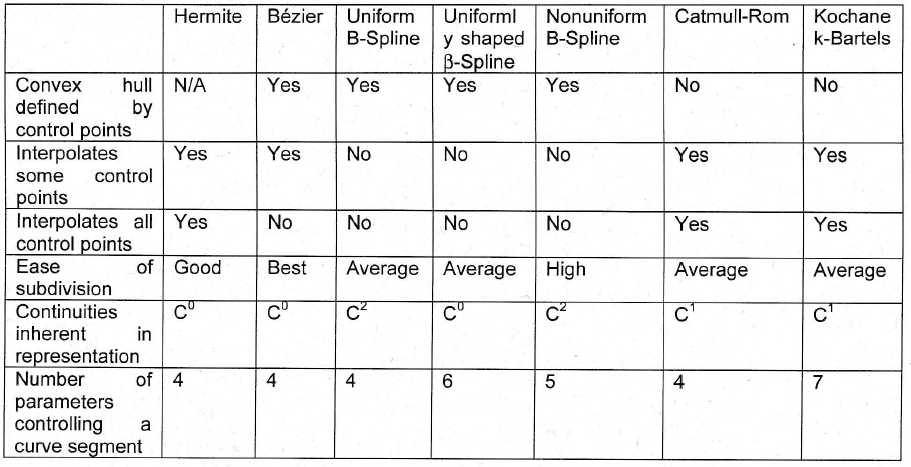
\includegraphics[scale=0.6]{3_25}

\subsubsection*{Approximating Splines}

\begin{itemize}
	\item If an approximating curve is described by control points, there is an additional requirement that the resulting curve has to be within the polygon shaped by the control points
	\item The shape is a complex polygon that encloses all control points like a rubber band
	\item If the control points are extreme points, they are part of the polygon; otherwise, they are inside of the polygon
	\item The complex shape allows a good control of the curve (guarantees the curve is always within the visible area)\\
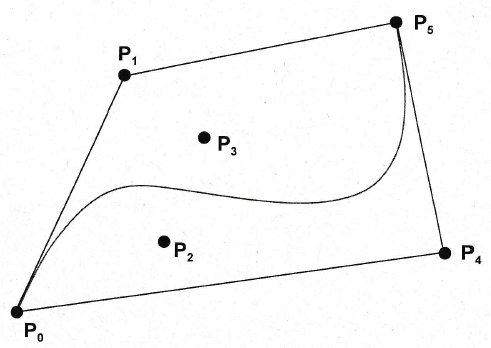
\includegraphics[scale=0.5]{3_26}
	\item B\'ezier Curve
	\begin{itemize}
		\item the base function is defined in a parametric form Q(t), t is a variable within [0, 1)
		\item the base function depends on the amount of control points; the whole curve is changed by just changing one point
		\item in addition to B\'ezier curve, also the first and last control point belong to the curve Q(t)
		\item always inside a complex polygon, because at least three control points are extreme points
		\item The Algorithm of de Casteljau: \\
		The base function of a B\'ezier curve can be calculated by the algorithm of de Casteljau\\
		idea: choose t and subdivide the first line b\textsubscript{0}b\textsubscript{1} at the distance t
		\begin{equation}
			b\textsubscript{0}\textsuperscript{1}(t) = (1-t)b\textsubscript{0}+t b\textsubscript{1}
		\end{equation}
		This process is repeated for the lines b\textsubscript{1}b\textsubscript{2} and b\textsubscript{2}b\textsubscript{3}, until in total three new points b\textsubscript{0}\textsuperscript{1}, b\textsubscript{1}\textsuperscript{1}, b\textsubscript{2}\textsuperscript{1} will result \\
		the calculation is repeated with the three new points and so on \\
		In general:
		\begin{equation}
			b\textsubscript{i}\textsuperscript{r}(t) = (1-t)b\textsubscript{i}\textsuperscript{r-1}+t b\textsubscript{i+1}\textsuperscript{r-1}
		\end{equation}
		\begin{equation}
			b\textsubscript{i}\textsuperscript{r}(t) = b\textsubscript{i}
		\end{equation}
		i = number of control points; i=0,...(n-r), r = number of lines; r=1,...,n
	\end{itemize}
	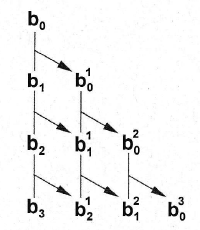
\includegraphics[scale=0.75]{3_29} 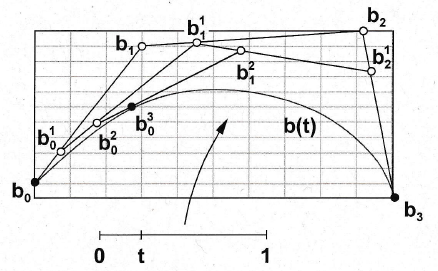
\includegraphics[scale=0.75]{3_30}
	\begin{itemize}
		\item For a better approximation of the curve, more control points have to be used which will increase the computing time
		\item The algorithm of de Castelijau can also be used, if more than four control points exist
		\item The number of control points(L+1) defines the kind of curve
		\item For L=3 (cubic B\'ezier curve), it is further elaborated and simplified as:
		\begin{equation}
			Q(t) = b\textsubscript{0}(1-t)\textsuperscript{3}+b\textsubscript{1}3t(1-t)\textsuperscript{2}+b\textsubscript{2}3t\textsuperscript{2}(1-t)+b\textsubscript{3}t\textsuperscript{3}
		\end{equation}
		\item Bernstein Polynomials: \\
		B\'ezier curves can be more easily calculated by using it; do not work recursively but directly deliver the result at the position t by using polynomial coefficients \\
		When (L+1) control points are given, the function is defined by:
		\begin{equation}
			Q(t) = \sum_{i=0}^Lb\textsubscript{i} B\textsubscript{i}\textsuperscript{L}(t)
		\end{equation}
		$$ B\textsubscript{i}\textsuperscript{L}(t) $$ is the Bernstein polynomial, which is defined as:
		\begin{equation}
			B\textsubscript{i}\textsuperscript{L}(t)= \textsubscript{L}C\textsubscript{i} (1-t)\textsuperscript{L-i}t\textsuperscript{i}, \quad L >=i
		\end{equation}
	\end{itemize}
	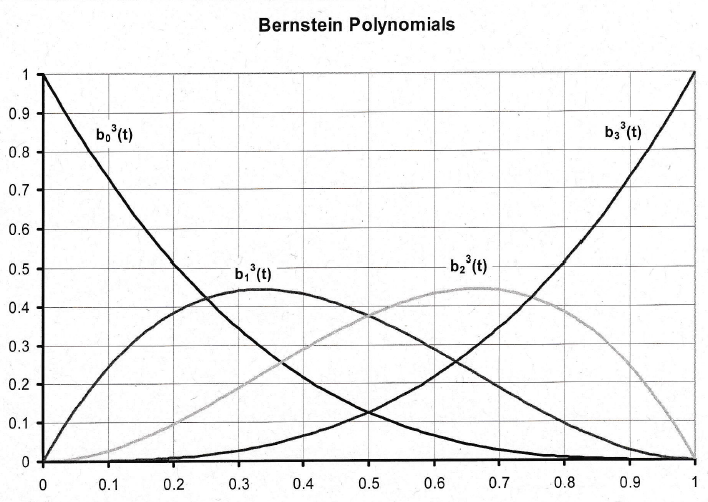
\includegraphics[scale=0.65]{3_31}
	\begin{itemize}
		\item If B\'ezier curves of a high degree are employed, it is difficult to keep the curve smooth
		\item Bernstein polynomials can also be calculated by a successive superposition of linear B\'ezier splines
	\end{itemize}
	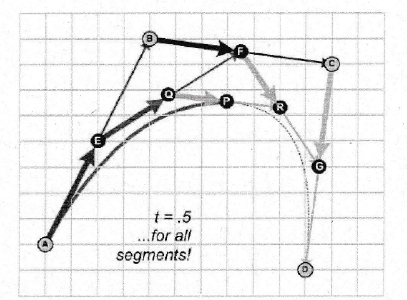
\includegraphics[scale=0.8]{3_32}
\end{itemize}

\subsubsection*{Interpolating Splines}

\begin{itemize}
	\item Boundary Representation - B-Rep
	\begin{itemize}
		\item Edge representations(or surface models or boundary representation) use 3D polygons to define the limiting surfaces of an object \\
		The limiting surfaces can be plain surfaces, but also surfaces of higher order \\
		It allows an exact mathematical description for many geometries, good approximation for the others
		\item B-Rep models consist of three object types: surfaces, edges, and corners
		\item To create on object out of the individual surfaces, the data structure must also contain a topological part(which defines the neighborhood of the surfaces) beside the normal geometric definition \\
		very common topological list contains 4 parts: a list of points/edges/surfaces/volumetric objects \\
		This list corresponds to a point-edge-surface model \\
		advantage: compact storage of all defining elements, since every point has to be stored only once
		\item The advantage of surface models consists in the complete availability of all topological information \\
		Surfaces, edges, and points can be stored as individual objects, which significantly increases the flexibility of the object \\
		one drawback: high calculation effort and complex network structure
	\end{itemize}
\end{itemize}

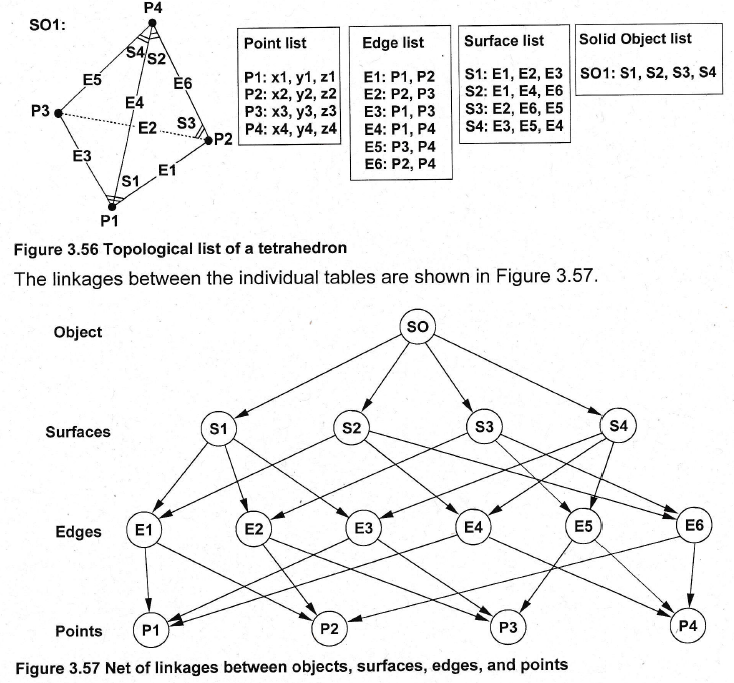
\includegraphics[scale=0.7]{3_56}

\subsubsection*{Volumetric Models}

\begin{itemize}
	\item The goal is to create objects that can be generally used (not only suitable for special applications)
	\item Only complete representations of physical objects are accepted
	\item Volumetric models can be distinguished into: \\
	cell models: 
\end{itemize}

\newpage
$$ \alpha \delta \Delta \delta \int_a^b f(x) \sum_{i=1}^n \text{exp}(-t) $$

\begin{equation}
	f(x) = \text{exp}(-t)
\end{equation}

\begin{align}
	A &= B \\
	&= C
\end{align}

\section{Chapter 4}

\end{document}
